\section{Our Method}
\label{sec:method}

The workflow of our method is illustrated in Figure~\ref{fig:pipeline}.  
From the fusion simulations, , we first precondition the data with the robust principal component analysis (RPCA)~\cite{CandesLMW11}, and then use the topology analyses to extract blobs as connected components of critical points (local minima/maxima).  The blobs are further tracked over different timesteps.  The dynamics of the blobs, such as birth/death/merge/split events are further visualized for fusion scientists to analyze the data.  


% We first load the output scalar electrostatic potential field from ADIOS I/O, 

\begin{figure}[!h]
  \centering
  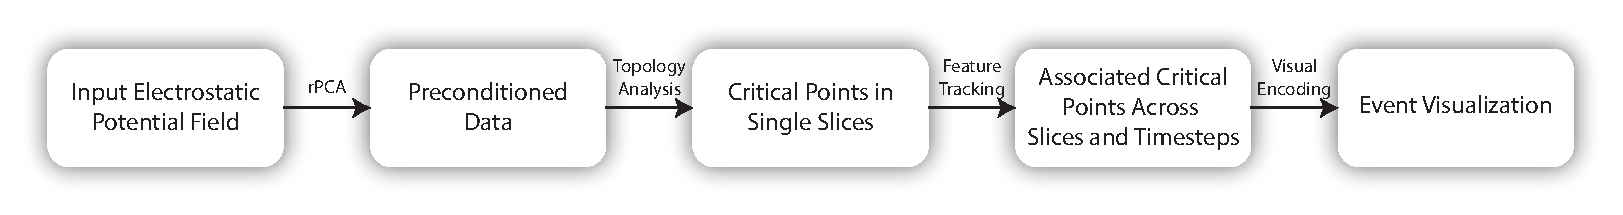
\includegraphics[width=\linewidth]{Figs/pipeline}
  \caption{The pipeline of our method.}
  \label{fig:pipeline}
\end{figure}


\subsection{Data Preconditioning}

We use the RPCA to precondition the time series data, in order to distinguish the moving and stationary patterns as ``foregrounds'' and ``backgrounds.''  Formally, the input data matrix $M$ can be decomposed as 

\begin{equation}
M = L_0 + S_0, 
\end{equation}

\noindent where $L_0$ has low rank and $S_0$ is a sparse perturbation matrix.  RPCA has been used to identify activities in video surveillance data, so that $L_0$ and $S_0$ correspond to the stationary background and moving features, respectively.  By preconditioning the input time series, we can detect the moving features for further blob tracking.  We are working with George Ostrouchov and Jong Choi from ORNL to generalize this technique to precondition the triangular mesh data.  


\subsection{Topology-based blob detection}

%\begin{figure}[!h]
%  \centering
%  \includegraphics[width=\linewidth]{Figs/blobs}
%  \caption{(a) Blob tracking over slices and time; (b) critical point tracking based on the combinatorial feature flow fields (image courtesy Reininghaus et al.~\cite{ReininghausKWH12})}
%  \label{fig:blob}
%\end{figure}

\begin{figure}[!h]
  \centering
  \includegraphics[width=\linewidth]{Figs/simplification2D}
  \caption{Topology simplification of a 2D slice with three different persistence thresholds: (a) 0, (b) 20, (c) 40.}
\end{figure}


As illustrated in Figure~\ref{fig:blob}(a), in our study, blob detection is defined as the extraction of critical points (local minima and maxima) in 2D slices; blob tracking is defined as associating blobs across different planes and different timesteps.  The critical point tracking is based on the combinatorial feature flow fields method~\cite{ReininghausKWH12}, which is a generalization of a feature flow field~\cite{TheiselS03} in the combinatorial sense.  We are also going to use merge tree theories to simplify the blob detection and tracking results~\cite{OesterlingHWMS17}.  3D visualizations will be provided to explore the spatiotemporal distributions of the tracked blobs.  

Topology simplifications.  



\subsection{Topology-based blob tracking}



\subsection{Event visualization}

\begin{figure}[!h]
  \centering
  \includegraphics[width=\linewidth]{Figs/events}
  \caption{Event visualization of blobs (image courtesy Scott Klasky, ORNL)}
  \label{fig:events}
\end{figure}

We are going to develop new visualizations for fusion scientists to understand the dynamics of the blobs.  We will define several different types of events, including birth, death, merge, and split to characterize the behaviors of blobs.  In our previous study of magnetic flux vortex tracking~\cite{GuoPPKG16, GuoPG17, PhillipsGPKG16, PhillipsPKG15}, we have already developed a graph-based representation of such events.  We are going to further generalize the previous methods to visualize the events in the XGC data.  

% 

% Critical point tracking~\cite{ReininghausKWH12}.

% 

% Feature flow fields~\cite{TheiselS03}. 
